%\chapter{Problema y Diseño Experimental}
\chapter{Descripción del problema}

En este capítulo se presenta el problema que se aborda con el algoritmo creado, así como las necesidades que surgen por el interés de identificar el aporte de este frente al panorama actual del campo en términos de rendimiento, las soluciones que existen para satisfacer dicha necesidad y cuál de ellas es la más adecuada.

\section{Introducción}

El problema que se va a abordar en este proyecto es el de la optimización de problemas de tipo combinatorio. 

\begin{definicion}
Un \textbf{problema de optimización combinatoria} se define como aquel en el que el conjunto de soluciones posibles es discreto. 
Es decir, se trata de un problema de optimización que involucra una cantidad finita o numerable de soluciones posibles.
\end{definicion}
Este tipo de problemas se diferencia de los problemas de optimización continuos, en los cuales el conjunto de soluciones posibles es infinito e incontable. 

Dentro del campo de la optimización combinatoria es común que la mayoría de los procesos de resolución de problemas no puedan garantizar la solución óptima, incluso dentro del contexto del modelo que se esté utilizando. 
Sin embargo, la aproximación al óptimo suele ser suficiente para resolver los problemas en la práctica. 

Con el fin de poder estudiar más a fondo el comportamiento de los distintos algoritmos que se han estado desarrollando era necesario elegir un problema determinado con el que trabajar. 
En nuestro caso, se ha elegido la generalización del problema comúnmente llamado ``problema de la mochila'' (\textit{Knapsack Problem} (KP)):  \textbf{\textit{Quadratic Knapsack Problem} (QKP)}. 

%Justificación de por qué hemos usado QKP
Antes de definir el problema, justificaremos por qué se ha elegido este problema. 
La primera razón, y posiblemente la más importante, es la ausencia de \textit{benchmarks} para problemas combinatorios \textit{expensive}, por lo que nos hemos visto obligados a crear el nuestro propio para un futuro. 
Ante este panorama también debemos encontrar un problema específico adecuado sobre el que trabajar desde cero y que resulte de interés. 
Como el objetivo inicial estaba relacionado con redes neuronales, buscamos un problema que puede tener representación binaria (\texttt{1} para la elección de elementos, \texttt{0} para el caso contrario). 
En este sentido, el QKP cumple con este requisito, además tiene interés añadido debido a que es un problema con restricciones y constituye una alternativa moderna de un problema clásico; además de que podemos generar instancias de este problema con distintos tamaños. 
Además, es un problema que tiene muchas aplicaciones en el mundo real en situaciones donde los recursos con distintos niveles de interacción tienen que distribuirse entre distintas tareas, por ejemplo, asignar compañeros de equipo a distintos proyectos donde las contribuciones de cada miembro se consideran de forma individual y por parejas. 
Por lo tanto, teniendo en cuenta la falta de \textit{benchmarks} y referencias, el QKP resulta ser una buena opción, ya que es un problema difícil, costoso y moderno. 


\section{Quadratic Knapsack Problem}
%The quadratic knapsack problem—a survey
Se procede a definir en profundidad dicho problema. 
En primer lugar, se tienen $n$ elementos donde cada elemento $j$ tiene un peso entero positivo $w_j$. 
Adicionalmente, se nos da una matriz de enteros no negativos de tamaño $n\times n$, $P = \{p_{ij}\}$, donde $p_{jj}$ es el beneficio asociado a elegir el elemento $j$ y $p_{ij}+p_{ji}$ es el beneficio que se alcanza si ambos elementos $i,j$, con $i<j$ son seleccionados. 
Consideramos que una combinación de elementos es una solución a QKP cuando peso el total (la suma del peso de todos los elementos seleccionados) no superan la capacidad máxima de la mochila dada, $c$. 
Así, el problema consiste el maximizar el beneficio total sin sobrepasar la capacidad máxima.

Por conveniencia en la notación, establecemos que $N=\{1,\dots,n\}$ denotará el conjunto de elementos. 
Representando la lista de elementos de forma binaria, $x_j$, para indicar si el elemento $j$ ha sido seleccionado (su valor será 0 si no ha sido seleccionado, 1 en caso contrario), el problema podrá ser formulado de la siguiente forma:
\begin{equation}
\begin{aligned}
  \text{maximizar} & \sum_{i\in N}\sum_{j\in N}p_{ij}x_ix_j \\
  \text{sujeto a } & \sum_{j\in N}w_jx_j \leq c\\
  & x_j\in \{0,1\}, j \in N 
\end{aligned}
\label{eq:QKP}
\end{equation}

Sin pérdida de generalidad, podemos suponer que:
\begin{itemize}
	\item $\max_{j\in N} w_j \leq c < \sum_{j\in N}w_j$
	\item La matriz de beneficios es simétrica, es decir, $p_{ij} = p_{ji}$, $\forall j > i$.
\end{itemize}

Una vez definido el problema, es fácil ver por qué es una versión generalizada del KP. 
KP se puede obtener a partir de QKP si $p_{ij} = 0$, para todo $i\neq j$. 
También se considera una versión restringida del \textit{Quadratic 0-1 Programming Problem} (QP), el cual se define como \ref{eq:QKP} sin la restricción de capacidad.

Como uno cabría esperar, debido a su generalidad, el QKP tiene un amplio espectro de aplicaciones. 
Witzgall \parencite{witzgallMathematicalMethodsSite1975} presentó un problema que surge en telecomunicación cuando un número de localizaciones para satélites tienen que ser seleccionados, tales que el tráfico global entre estas estaciones se maximice y la limitación de presupuesto se cumpla; este problema resulta ser un QKP. 

En tanto que QKP es un problema $\mathcal{NP}-hard$, no podemos esperar encontrar una aproximación totalmente polinómica a no ser que $\mathcal{NP}=\mathcal{P}$. 
Sin embargo, Rader y Woeginger \parencite{raderjrQuadraticKnapsackProblem2002}
desarrollaron un esquema de aproximación en tiempo completamente polinómico (FPTAS, \textit{Fully polynomial-time approximation scheme}) para el caso especial donde todos los beneficios $p_{ij}\geq 0$. 
También probaron que si el problema tiene coeficientes de la función objetivo positivos y negativos, entonces el problema es fuertemente $\mathcal{NP}-hard$, por lo que no podemos esperar encontrar ningún FPTAS (a no ser que $\mathcal{NP}=\mathcal{P}$).

\section{Datos del problema}

Utilizaremos 97 archivos de datos generados aleatoriamente de \href{http://cedric.cnam.fr/~soutif/QKP/QKP.html}{(QKP) \textit{instances}}\footnote{http://cedric.cnam.fr/~soutif/QKP/QKP.html}, los cuales se pueden distribuir de forma que se indica en la Tabla \ref{DatosProblema}.

\begin{table}[h]
\caption{Datos del Problema}
\label{DatosProblema}
\begin{tabular}{|c|c|c|}
\hline
\rowcolor[HTML]{F7EAC7} 
\multicolumn{1}{|l|}{\cellcolor[HTML]{F7EAC7}Número de variables} & \multicolumn{1}{l|}{\cellcolor[HTML]{F7EAC7}Densidad} & \multicolumn{1}{l|}{\cellcolor[HTML]{F7EAC7}Número de archivos} \\ \hline
\rowcolor[HTML]{DDFDFF} 
\cellcolor[HTML]{DAE8FC}                                          & 25\%                                                  & 10                                                              \\ \cline{2-3} 
\cellcolor[HTML]{DAE8FC}                                          & 50\%                                                  & 10                                                              \\ \cline{2-3} 
\rowcolor[HTML]{DDFDFF} 
\cellcolor[HTML]{DAE8FC}                                          & 75\%                                                  & 10                                                              \\ \cline{2-3} 
\multirow{-4}{*}{\cellcolor[HTML]{DAE8FC}n = 100}                 & 100\%                                                 & 9                                                              \\ \hline
\rowcolor[HTML]{DAE8FC} 
\cellcolor[HTML]{DDFDFF}                                          & 25\%                                                  & 9                                                              \\ \cline{2-3} 
\cellcolor[HTML]{DDFDFF}                                          & 50\%                                                  & 10                                                              \\ \cline{2-3} 
\rowcolor[HTML]{DAE8FC} 
\cellcolor[HTML]{DDFDFF}                                          & 75\%                                                  & 10                                                              \\ \cline{2-3} 
\multirow{-4}{*}{\cellcolor[HTML]{DDFDFF}n = 200}                 & 100\%                                                 & 10                                                              \\ \hline
\rowcolor[HTML]{DDFDFF} 
\cellcolor[HTML]{DAE8FC}                                          & 25\%                                                  & 9                                                              \\ \cline{2-3} 
\multirow{-2}{*}{\cellcolor[HTML]{DAE8FC}n = 300}                 & 50\%                                                  & 10                                                              \\ \hline
\end{tabular}
\end{table}

Se entiende como ``densidad'' al porcentaje de beneficios combinados positivos, es decir, $p_{ij} > 0$. 
Particularmente, QP tendría densidad 0\%.

Ahora bien, todos los archivos tienen el mismo formato, lo cual resulta útil para definir funciones capaces de obtener los datos más relevantes para nuestros algoritmos. 
En primer lugar, mencionar que todos los archivos de datos tienen el mismo formato de nombre:
\begin{equation*}
\text{jeu\_}n\text{\_}d\_x\text{.txt}
\end{equation*}
donde $n$ representa el número de variables que contiene, $d$ la densidad y $x$ el número asociado a dicha instancia. 

Dentro de cada archivo de datos se sigue el siguiente formato para representar los datos:
\begin{itemize}
	\item La referencia de la instancia: Su nombre.
	\item El número de variables ($n$)
	\item Los coeficientes lineales de la función objetivo $p_{jj}$
	\item Los coeficientes cuadráticos $p_{ij}$: representados en líneas
	\item Una línea en blanco
	\item 0 si la restricción es de tipo $\leq$, lo cual siempre va a ocurrir ya que estamos considerando instancias QKP.
	\item La capacidad $c$ de la mochila.
	\item Los coeficientes de capacidad/peso, $w_j$.
	\item Algunos comentarios.
\end{itemize}

%Introducir algún ejemplo?
Un ejemplo breve con 10 variables de qué contendría un archivo y cómo analizarlo sería el siguiente:

\begin{figure}[H]
		\centering
		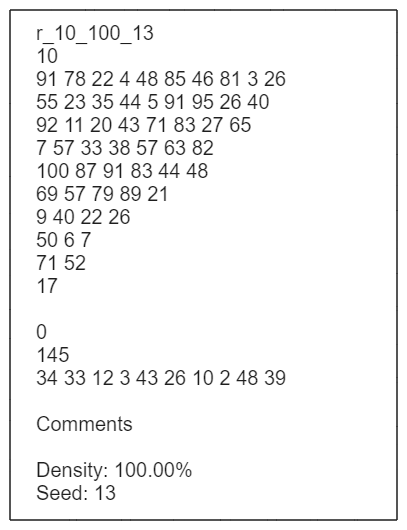
\includegraphics[scale=0.5]{imagenes/ejemploInstancia.png}
        \caption{Ejemplo de instancia de problema}
        \label{fig:ejemploInstancia}
\end{figure}

En este caso se tiene:
\begin{itemize}
	\item La referencia de la instancia (r\_10\_100\_13)
	\item El número de variables: 10
	\item Los coeficientes lineales de la función objetivo $p_{ii}$: 91 78 22 4 48 85 46 81 3 26
	\item Los coeficientes cuadráticos de la función objetivo $p_(ij)$: la matriz triangular
	\item Tras la línea en blanco tenemos un 0 que representa el tipo de restricción (todas las instancias con las que trabajamos en este caso tienen este tipo de restricción). 
	\item La capacidad total: 145.
	\item La capacidad que necesita cada variable $w_i$: 34 33 12 3 43 26 10 2 48 39
	\item Comentarios:
	\begin{itemize}
		\item La densidad: 100.00\%. Que la podemos obtener de la propia referencia, por lo que no nos es de mucha utilidad este dato. 
		\item La semilla: 13. Como se explicará más adelante, utilizaremos varias semillas con el fin de que los resultados sean reproducibles y poder utilizar tests estadísticos. Por lo tanto, tampoco nos es de mucha utilidad este dato. 
	\end{itemize}
\end{itemize}

